% This chapter will serve as an introduction to dark-matter physics
% and a little bit of neutrino physics

\chapter{Introduction}
	\label{chap:IntroChapter}

	% Set the context for the experiment a bit, why MJ can look for dark matter.  
	The \MJ~experiment experiment will search for the rare process of 
neutrinoless double-beta decay ($\nonubb$) to determine characteristics of the neutrino.  The 
choice of detector technology, p-type point contact germanium detectors, 
will also allow the experiment to search for dark matter.  
The following outlines the reasons behind using this technology and focuses on the
additional physics questions beyond those related to neutrinos which may be answered with these detectors.

	\section{Neutrinos and neutrinoless double-beta decay ($\nonubb$)}
	
	Neutrinos have provided evidence for physics beyond the Standard Model: 
neutrino oscillation experiments have shown that neutrinos are massive but
cannot determine the absolute neutrino mass scale or the nature of the neutrino
mass (see, e.g.~\cite{Mes04}).  Neutrinoless double-beta decay ($\nonubb$) is a
process which, if discovered, would imply that the neutrino is its own
antiparticle (a so-called `Majorana' particle) and would define the neutrino
mass scale.  $\nonubb$ could occur in several even-even nuclei (e.g.~$^{48}$Ca,
$^{76}$Ge, $^{130}$Te, $^{136}$Xe, etc.) otherwise stable against
single-beta decay and is characterized by the emission of two electrons with
total kinetic energy equal to the Q-value of the reaction, $\qval$.  For example:

		\begin{equation}
		(Z,A) \rightarrow (Z+2,A) + e^- + e^-
		\end{equation} 

where the Q-value is the mass difference $M(Z,A)-M(Z+2,A)-2m_e$.  The signal, therefore, 
is the deposition of energy in a detector equal to $\qval$.
A schematic of a possible lepton-number-violating mechanism for neutrinoless double-beta
decay is shown in Figure~\ref{fig:DBDK}.  Assuming left-handed currents and
that the decay is dominated by the exchange of a light massive Majorana
particle, the half-life of $\nonubb$ can be related to the effective mass of
the neutrino by:

		\begin{equation}
		\left( T_{1/2}^{0\nu}\right)^{-1} = G^{0\nu} |M^{0\nu}|^2 \langle m_{\nu_{\beta\beta}} \rangle^2  
		\end{equation} 

where $G^{0\nu}$ refers to an exactly calculable phase-space integral, 
$|M^{0\nu}|^2$ is a nuclear matrix element, and $\langle m_{\nu{\beta\beta}}\rangle$
is the effective neutrino mass.  $^{76}$Ge currently holds the best limit for
the $\nonubb$ half-life: $T^{0\nu}_{1/2}\geq 1.6\times10^{25}$~\cite{Bau99}.
Several review articles exist outlining the current theoretical and
experimental landscape (see e.g.~\cite{Ell02,Bara07}).  
Two-neutrino double-beta decay ($\twonubb$) is a related 
decay that can exist in the same nuclei allowed to undergo $\nonubb$:  

		\begin{equation}
		(Z,A) \rightarrow (Z+2,A) + e^- + e^- + \bar{\nu}_e + \bar{\nu}_e
		\end{equation}

The $\twonubb$ process has been seen in several nuclei including $^{76}$Ge and has
a half-life for these nuclei around $T^{2\nu}_{1/2}\sim10^{20}$~yrs.  

		\begin{figure}
			\centering
			\def\figheight{0.4\textheight}
			 \subfigure[$\twonubb$] {
			 	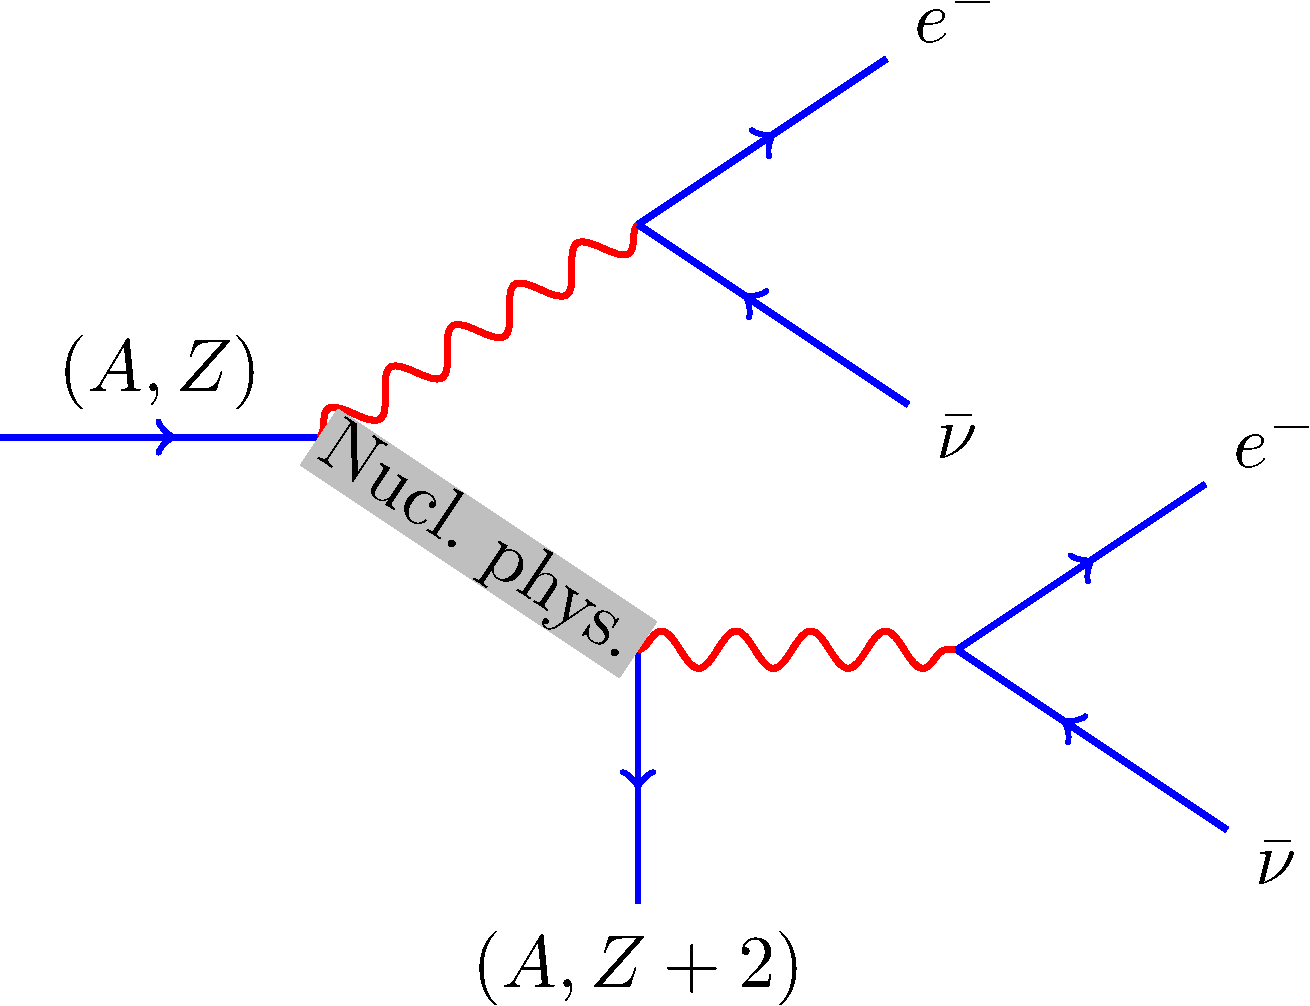
\includegraphics[height=\figheight]{2nubbDecay}
			}
			\subfigure[$\nonubb$]{
				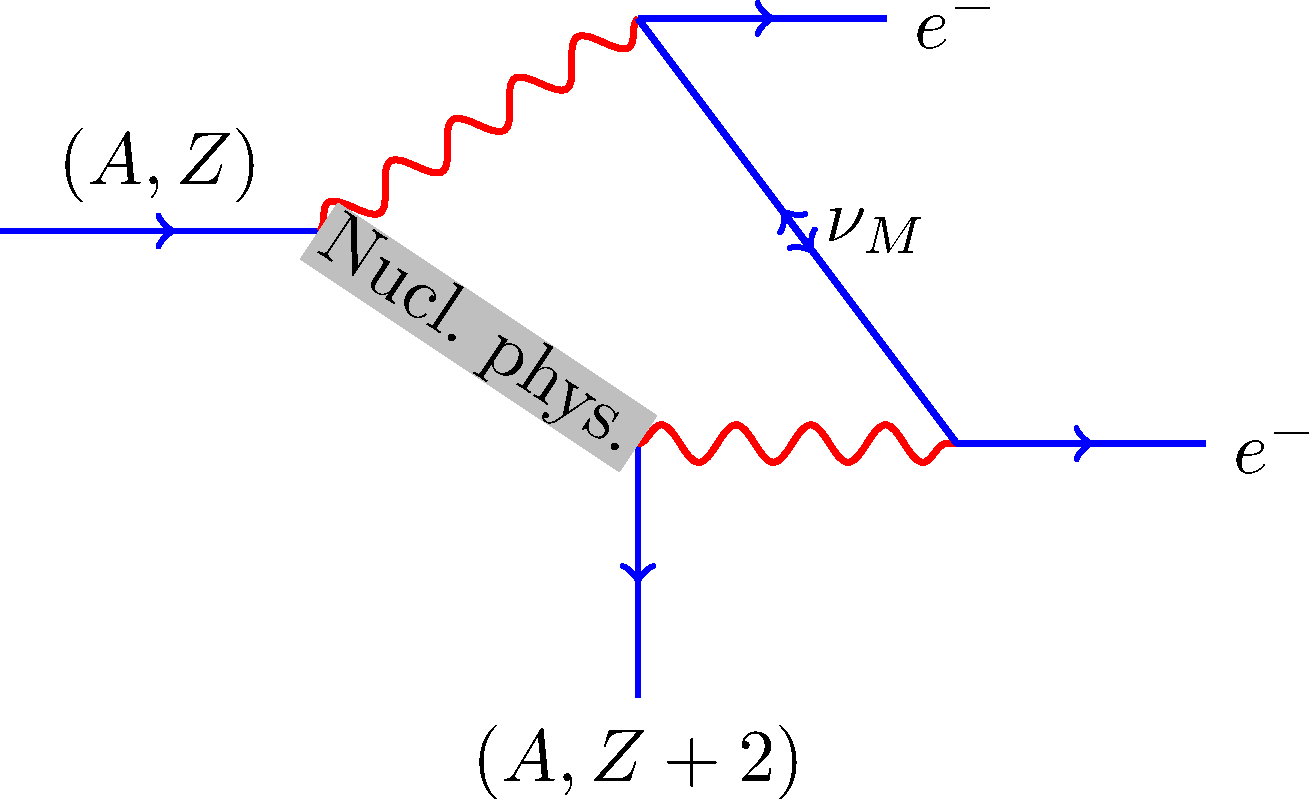
\includegraphics[height=\figheight]{0nubbDecay}
			}
		\caption[Schematic of $\twonubb$ and $\nonubb$ decays.]{Schematic figure of the two types of double-beta decay, 
		the 2$\nu$ mode and the 0$\nu$ mode.  
			In this schematic, the 0$\nu$ mode is mediated through the exchange of a virtual Majorana neutrino, $\nu_{M}$.}
		\label{fig:DBDK}
		\end{figure}
 

	
	\section{The \MJ\ experiment}
	\label{sec:MJExperiment}
	
The search for a rare process such as $\nonubb$ necessarily involves maximizing the magnitude of the expected signal while
simultaneously reducing backgrounds that may mimic the sought-after process.  
The \MJ~experiment proposes to search for $\nonubb$ in \gersevensix~using high-purity
germanium as both source and detector, thereby maximizing a possible signal from $\nonubb$. 
The first stage of this experiment will involve the deployment of 20-40~kilograms of germanium in a arrayed fashion in a \minmod~module with the goal to determine
the feasibility of scaling up to the 1-tonne scale.  To achieve this, the \MJ~experiment seeks to demonstrate less than
1~background count per year per tonne of enriched material in the
region-of-interest, a $\sim4$~keV window around the $\beta\beta$-decay
Q-value of $^{76}$Ge (2039~keV).  Low-capacitance, low-noise p-type point contact (\ppc)
detectors will be deployed in these modules to take advantage of characteristics which make 
them beneficial for rare-process searches in general and for looking for $\nonubb$ in particular.  These characteristics and other details about \ppc~detectors will be discussed in Section~\ref{sec:PPCDets}.  

To achieve its background goals, the \MJ~experiment will employ standard techniques for background reduction including: creation of detector mounts, cryostats, and other components close to the detectors using ultra-clean electroformed copper and other radiopure materials; use of passive shielding against external radiation including a lead shield for gamma radiation and a borated polyethylene shield for the moderation of cosmic-ray-induced neutrons; use of active shielding (vetos) against cosmic-ray muons; and deployment of the module underground in the Deep Underground Science and Engineering Lab (DUSEL) at Homestake, South Dakota, for moderation of cosmic-ray muons.  Engineering drawings given in Figures~\ref{fig:MJEngDrawing1} and~\ref{fig:MJEngDrawing2}shows both the cryostat design and the expected shield construction, and indicates the modular design of the experiment; additional, independent cryostats may be deployed within the same shield geometry.  
% FixME update
The expected sensitivity of this first stage, 
assuming 3 years with 30~kg of enriched material or 90~kg-yr of $^{76}$Ge
exposure, is T$_{1/2}\geq 10^{26}$.  
%Further information on the
%\MJ~experiment can be found in technical documents \footnote{Available:
%http://majorana.npl.washington.edu/general.php}. 

	
		\begin{sidewaysfigure}
			\centering		
			\def\figheight{0.45\textheight}
			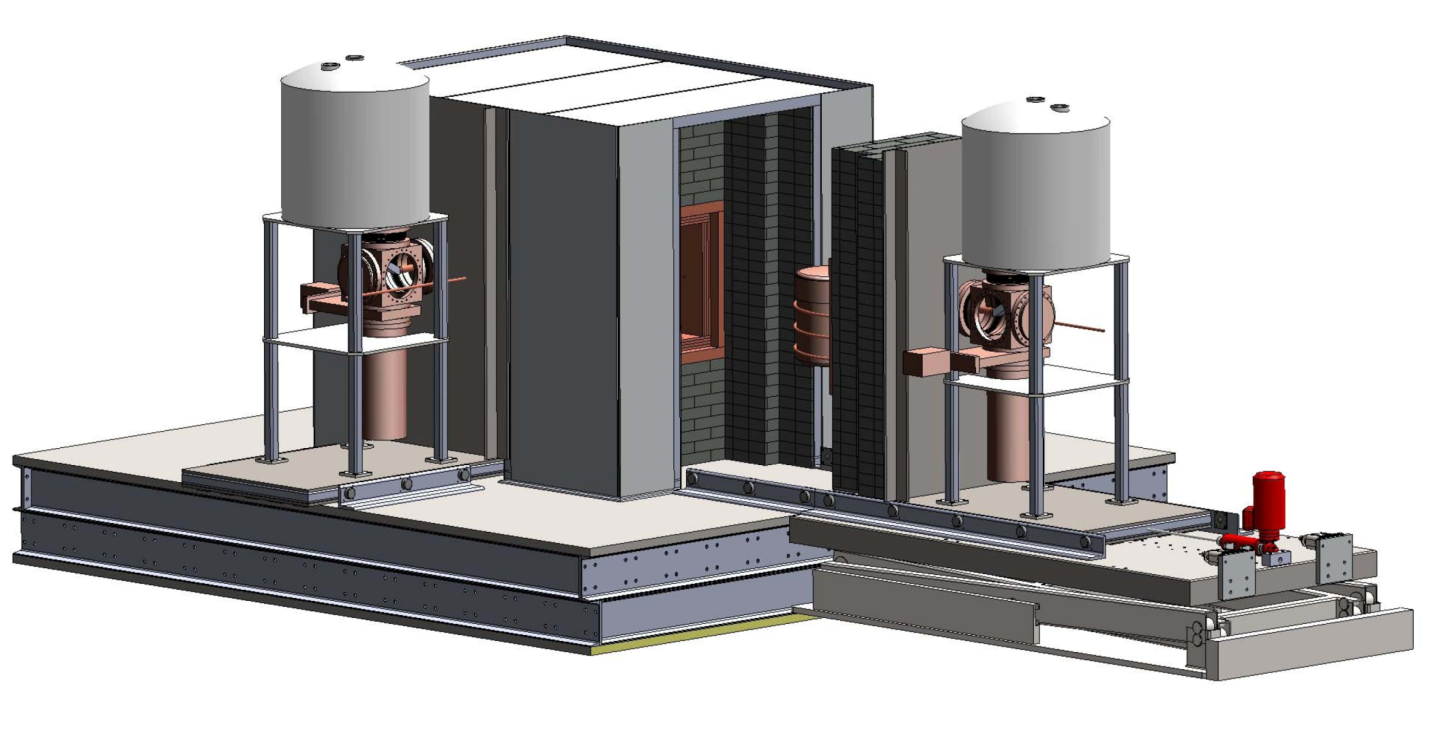
\includegraphics[height=\figheight]{ShieldDesign}
			\caption[\MJ~\minmod~shield geometry]{\MJ~\minmod~shield geometry.  The modular design of the shield will 
			enable a phased deployment of cryostats, allowing sets of detectors to be easily added after initial commissioning of the 
			experiment.}
			\label{fig:MJEngDrawing2}
		\end{sidewaysfigure}
	
		\begin{figure}
			\centering		
			\def\figheight{0.45\textheight}
			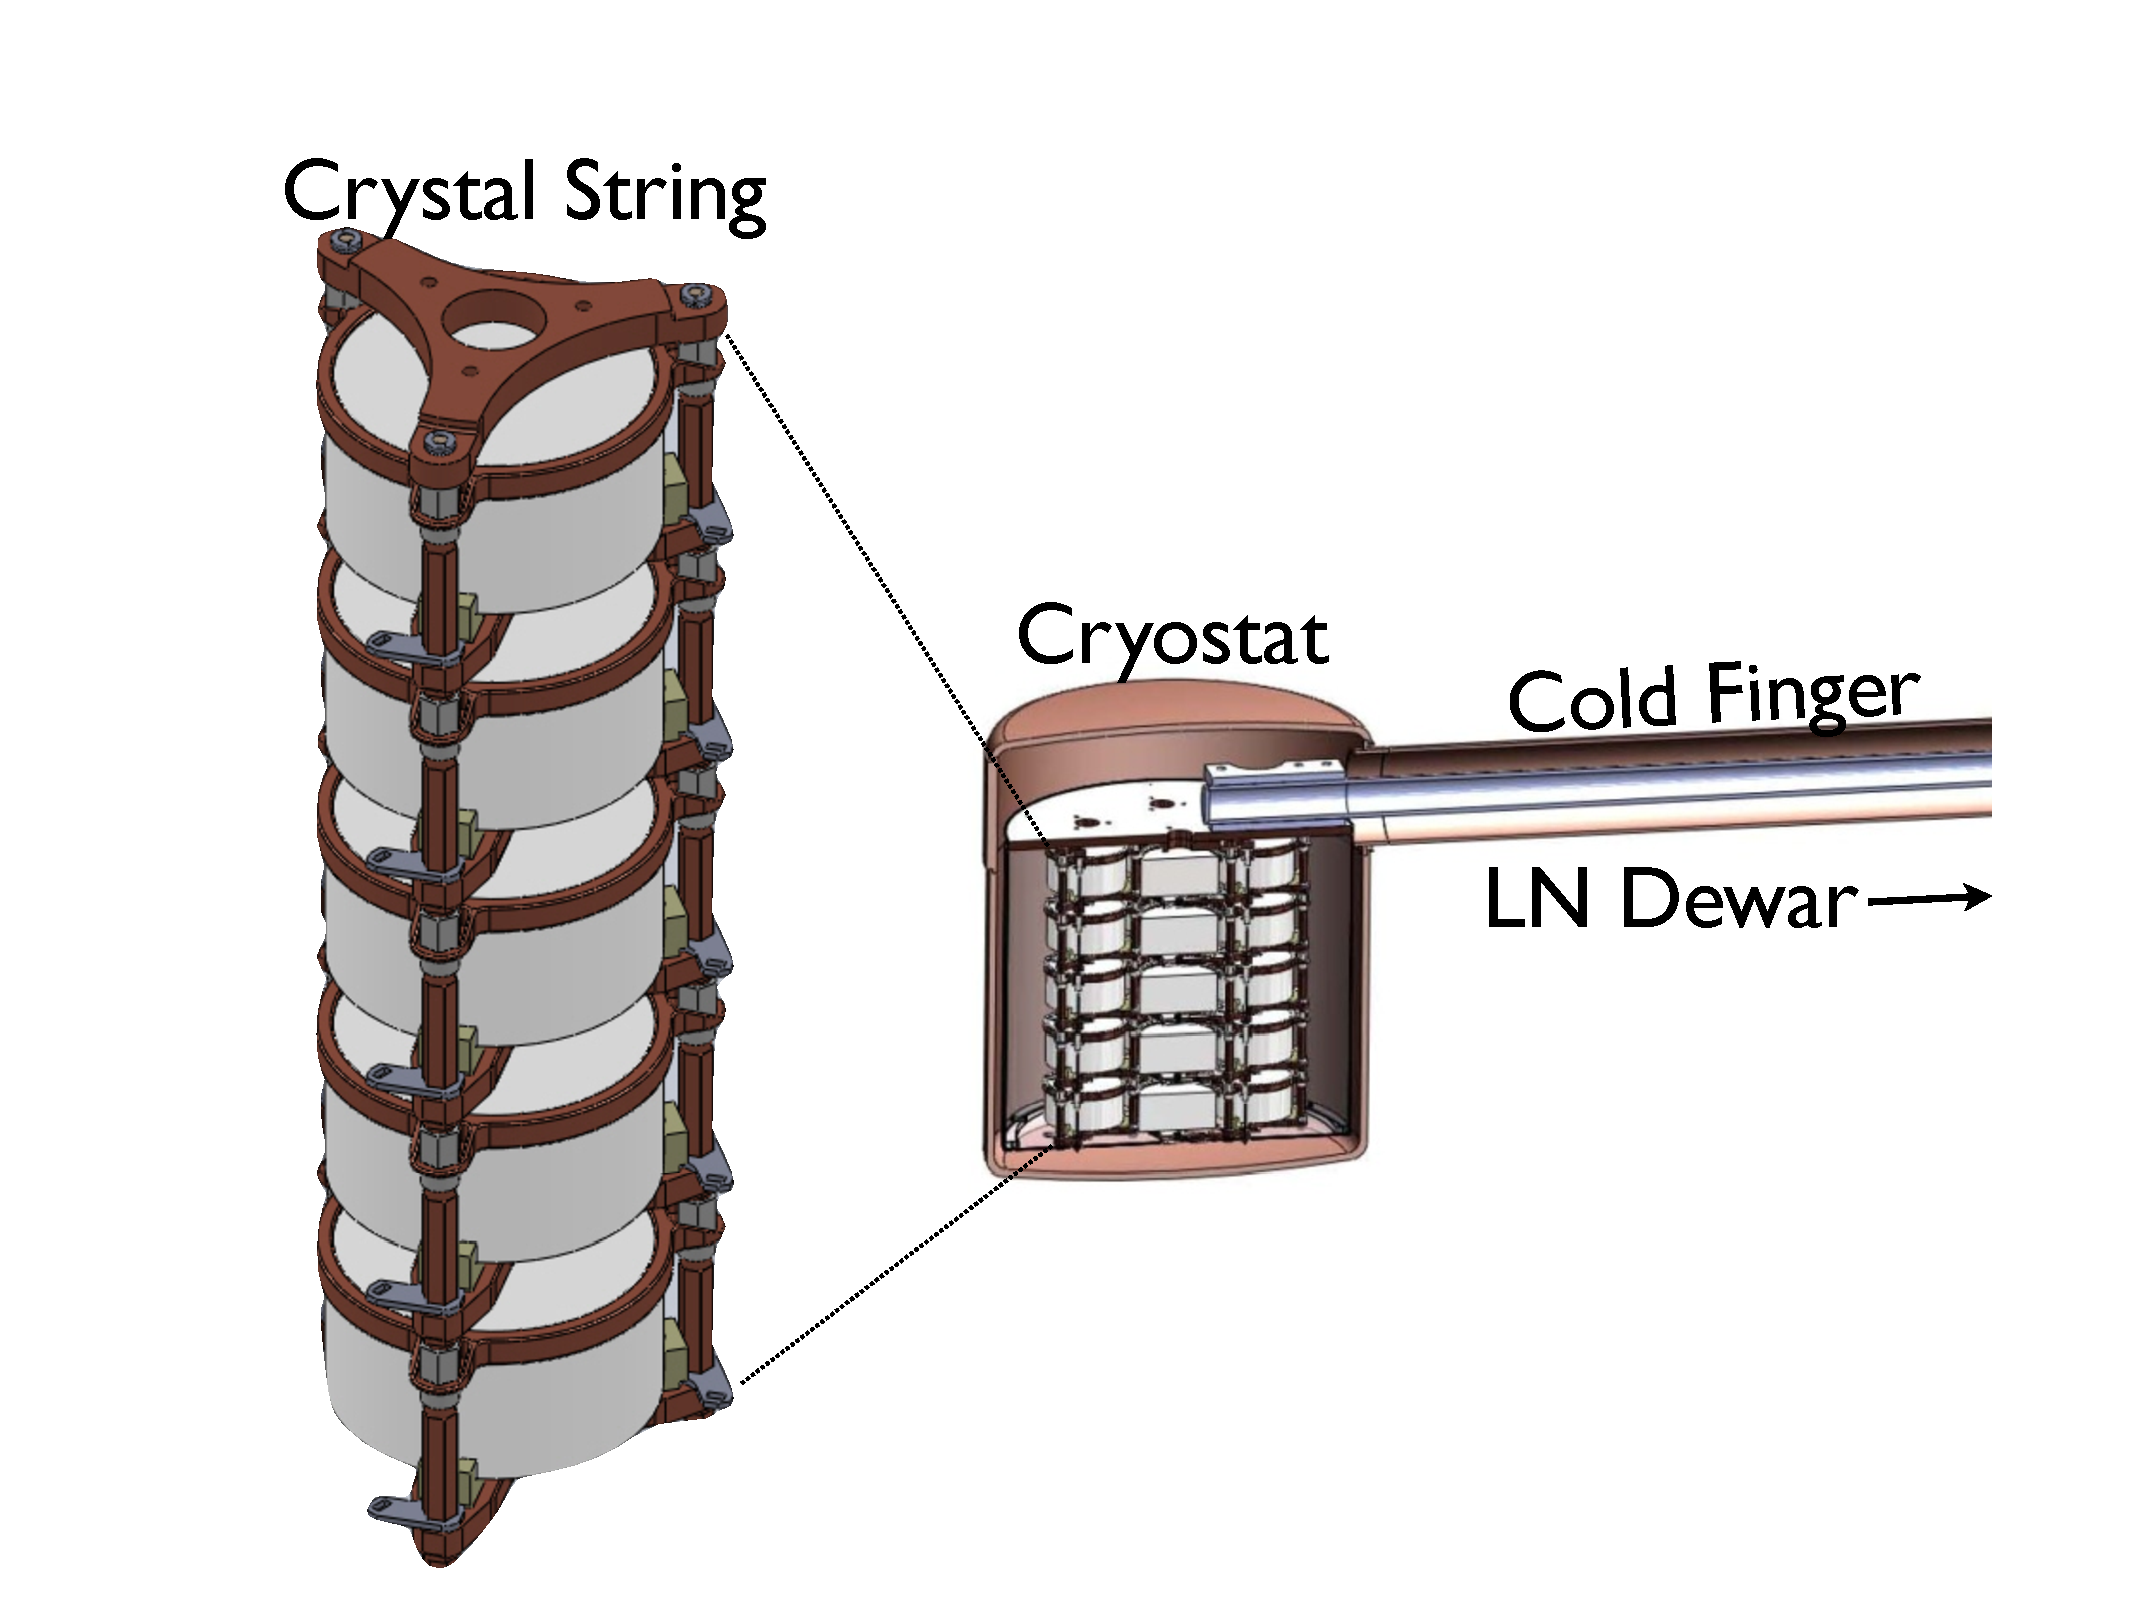
\includegraphics[height=0.9\textwidth]{CrystalCryostatDesign}
			\caption[\MJ~\minmod~cryostat and crystal string geometry]{\MJ~\minmod~cryostat and crystal string geometry, each
			crystal string houses 5~p-type point-contact germanium detectors.}
			\label{fig:MJEngDrawing1}
		\end{figure}

	
	\section{P-type point contact (\ppc) germanium detectors}
	\label{sec:PPCDets}

  P-type point-contact (\ppc) germanium detectors are an exciting detector
technology whose characteristics provide powerful tools in the search for
$\nonubb$ and enable searches for other rare physics processes at low energy, e.g.~dark matter.  
The electrode geometry of \ppc~detectors significantly reduces the
capacitance, reducing the energy threshold and enhancing the detector's
ability to detect low-energy ($\sim100$~eV) processes.  Figure~\ref{fig:PPCGeom} shows a picture of the geometry of this detector in comparison to a standard semi-coaxial crystal.  In addition to improving the electronic response of the detector, the crystal geometry also yields a weighting field strongly peaked at the readout electrode.  This means that as charge drifts to the p contact after being created from energy deposition in the crystal (e.g.~from a physics interaction), no signal will be induced in the contact until the drifting charge is very near (within $\sim1$~cm of) the contact.  Additionally, charge drift times are increased by the longer drift paths.  These two characteristics coupled together improve the ability to distinguish between charge originating from one point in the crystal or from multiple sites in the detector.

An n-type detector with a point-contact geometry was developed by Luke et
al.~in 1989, demonstrating detector capacitance on the order of
1~pF~\cite{Luke89}.  With such a low capacitance and therefore a low-energy
threshold this detector was seen as a potential tool for dark matter detection, but this detector 
exhibited poor energy resolution due to incomplete charge collection attributed to charge-trapping effects.  
		\begin{figure}
			\centering
			\subfigure[Point-contact geometry.]{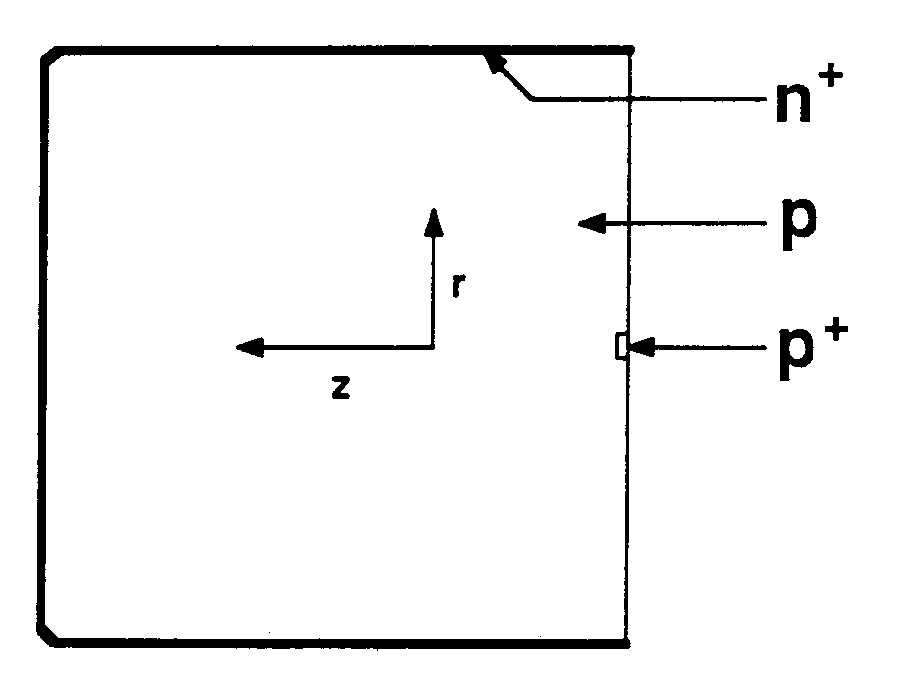
\includegraphics[height=0.2\textheight]{LukePPC}}
			\subfigure[Semi-coaxial geometry.]{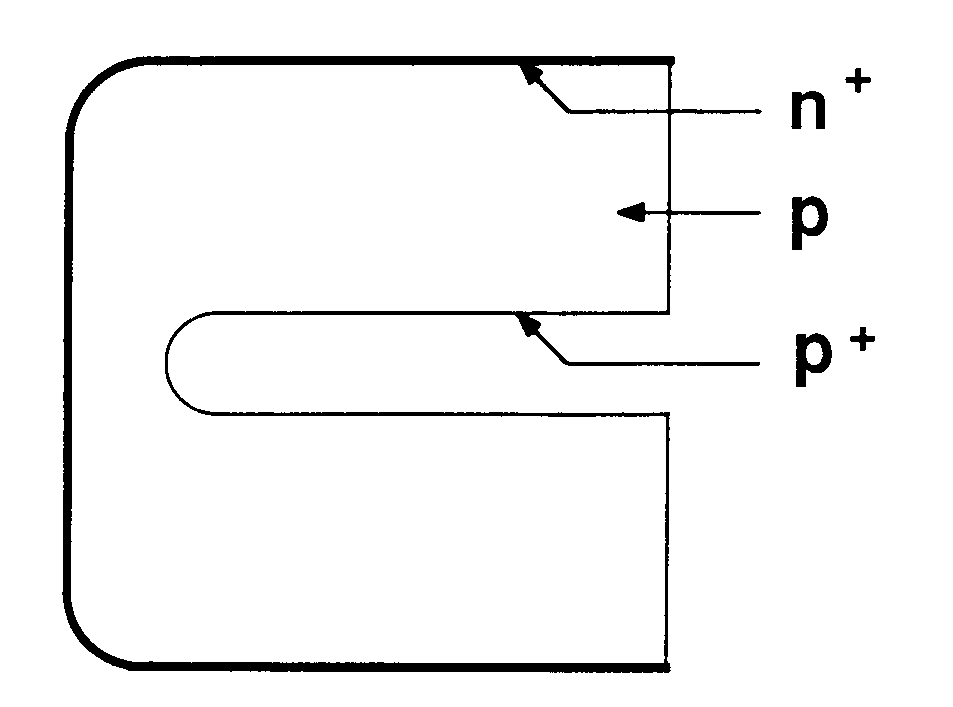
\includegraphics[height=0.2\textheight]{LukeCoax}}
			\caption[Ge detector geometry comparison: \ppc~and semi-coax.]{The left figure depicts the point-contact geometry, the right figure a conventional 
			         semi-coaxial geometry.  Figure adapted from~\cite{Luke89}.  The small diameter of the p contact in the
			          \ppc~detector reduces the capacitance of the detector improving the intrinsic noise characteristics.}
			\label{fig:PPCGeom}
		\end{figure}
  In 2007, Barbeau et al.~presented a new detector with a point-contact 
geometry, departing from previous convention by creating it out
of p-type material~\cite{Barb07}.  The reason for this
change was to take advantage of the reduced sensitivity of p-type crystals to electron trapping in germanium.  
Because p-type crystals collect holes instead of electrons at the p contact of the crystal, they are less likely to 
see a degradation of signal from electron trapping~\cite{Hull:2005p2207}.
With these changes, Barbeau et al.~demonstrated
a resolution comparable to conventional semi-coaxial germanium detectors and
an energy threshold of 330~eV making them an excellent candidate for double-beta decay searches.  
Other work with these detectors has supported these conclusions (see e.g.~\cite{Hull:2008p2206,Aalseth:2008aa}).
%Additionally, using a collimated $^{241}$Am gamma source (59.5~keV), they demonstrated differences in pulse rise-times based upon position of interaction (see Figure~\ref{fig:MeasPulses}).   

%\begin{figure}
%\begin{center}
%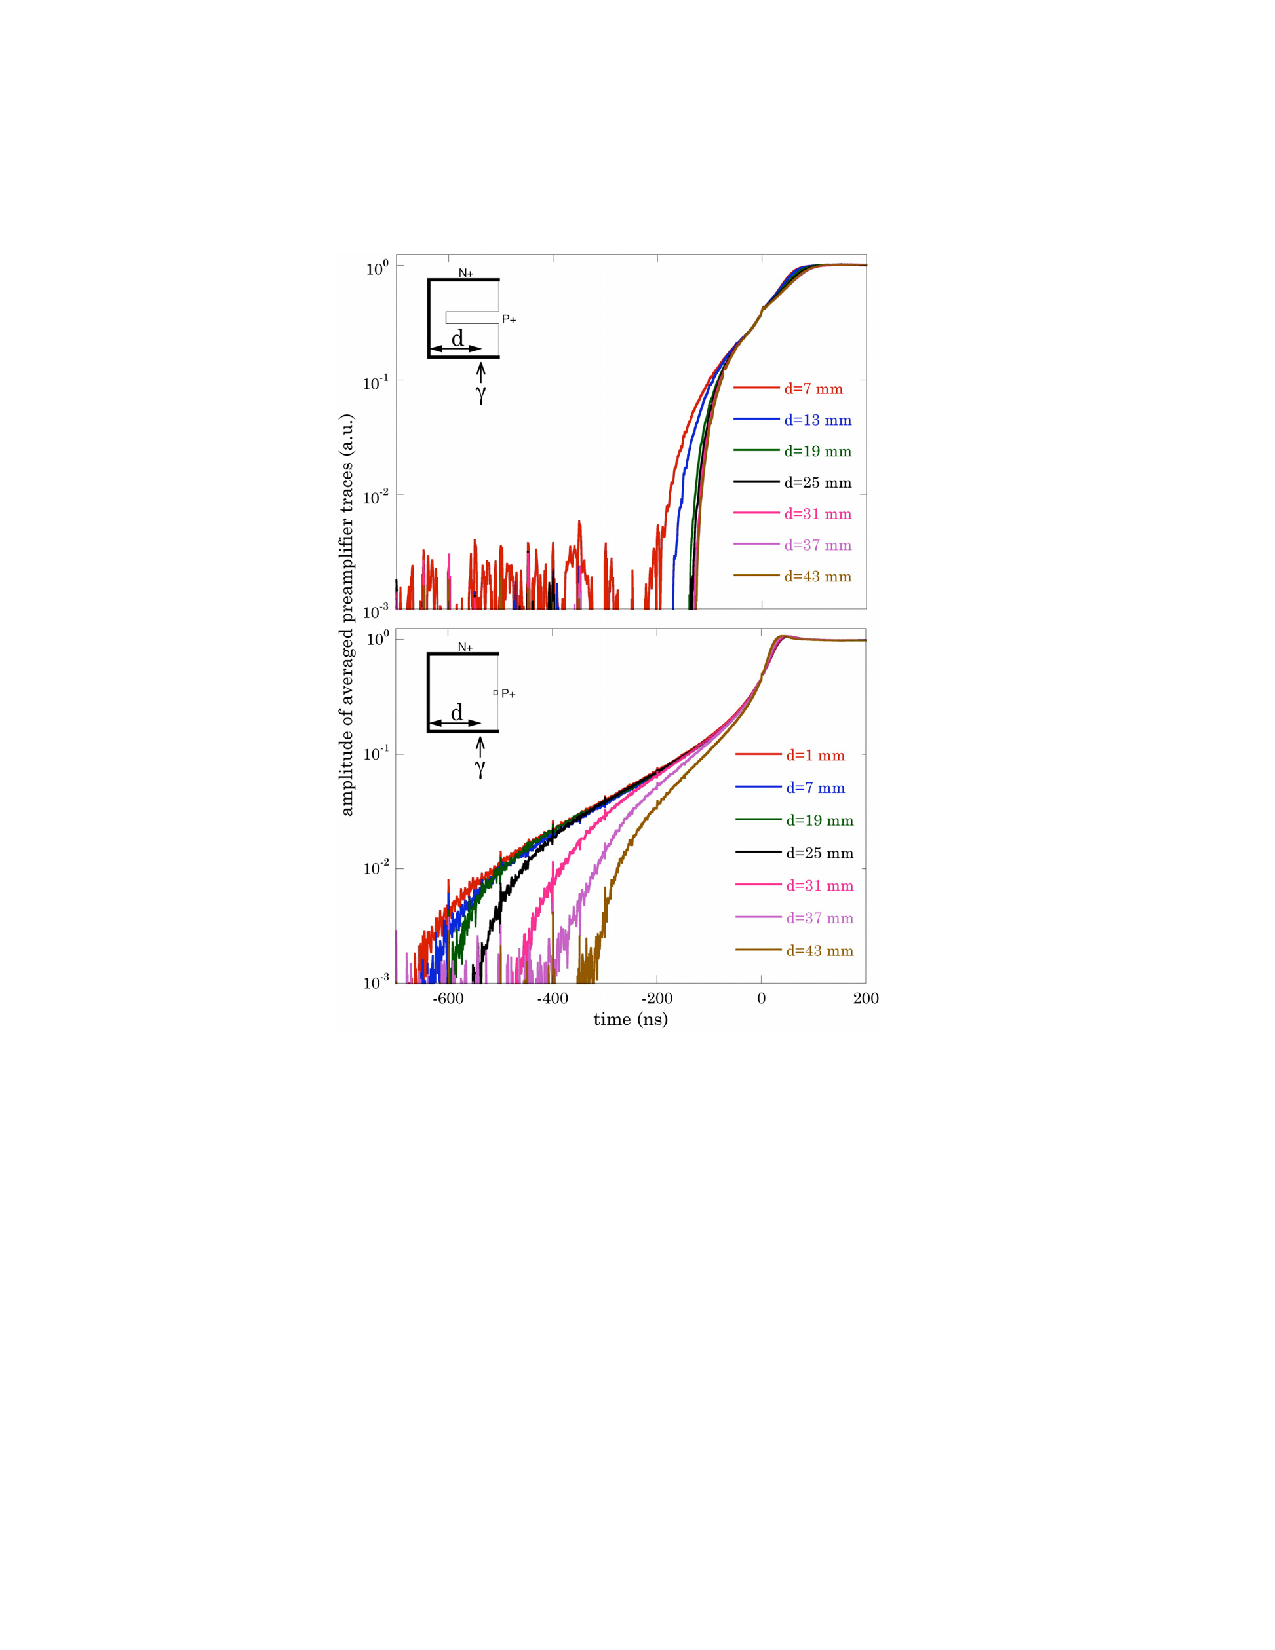
\includegraphics[width=0.8\textwidth]{BarbPPC}
%\caption{Pulses from a collimated ${241}$Am gamma source incident upon the surface
%         of a conventional semi-coax detector (top) and a p-type point-contact (bottom).
%         The expansion of the charge collection time in the \ppc~detector versus
%         the conventional semi-coax detector is evident.  (Figure from~\cite{Barb07}.)}
%\label{fig:MeasPulses}
%\end{center}
%\end{figure}

	\section{\ppc~detectors for the \MJ~experiment}

For the proposed \MJ~experiment, the characteristics of the \ppc~detector
will aid in the reduction of backgrounds and in enhancing the physics reach of
the experiment.  Since $\nonubb$ is an inherently single-site event, cutting out
multi-site events during data analysis provides a powerful background reduction
tool.  For conventional semi-coaxial detectors, various tools have been developed
to tag multi-site events based upon the shape of the measured pulse (see,
e.g.~\cite{Aal00}).  The expansion in time
of charge collection in \ppc~detectors makes distinguishing multi-site events easier and improves the efficiency for single-site acceptance vs. multi-site rejection of a pulse-shape analysis routine (see~\cite{Budjas:2009zu,Ren10}).

To improve the bandwidth of the detector readout it is necessary to
place front-end preamplification electronics (e.g.~field-effect transistors) nearby the detectors
inside the detector cryostat.  As with any low-background 
experiment the increase of material (and especially material close to
sensitive detectors) introduces potential radioactivity that could
increase background.  The single-contact nature of the \ppc~requires only one
front-end per crystal, thus reducing the material inside the cryostat and possibly
softening radiopurity requirements.

Cosmogenically-produced $^{68}$Ge is a significant background
source for the \MJ~experiment, decaying first via electron capture to $^{68}$Ga
(T$_{1/2}=271$~d) and then to $^{68}$Zn (Q=2921~keV, T$_{1/2}=68$~m).  The
initial decay is characterized by the emission of Auger electrons and/or soft x-rays
summing to the orbital energy of the captured electon (e.g.~1.3~keV for L-capture, 10.3~keV for K-capture) 
and it is possible to use these to tag the $^{68}$Ge decay.  A time cut can then be introduced to veto events
occurring within a few $^{68}$Ga lifetimes to mitigate background from that
decay without seriously affecting detector live time.   \ppc~detectors have an
improved sensitivity to low-energy physics because of their low noise and 
low-energy threshold and so could significantly enhance the tagging of the
$^{68}$Ge decay.  

Though characteristics of \ppc~detectors will prove useful in searching for
$\nonubb$, the low-energy threshold will also
expand the physics reach of the \MJ~experiment.  Access to low energies will 
make the \minmod~sensitive to low-energy nuclear recoils and enhance its capacity as a dark matter
detector.  The functionality and usefulness of the \ppc~detector as a tool for dark
matter searches is considered in much more detail 
throughout the remainder of this dissertation.


%The low energy threshold and low noise of the \ppc~detector won't necessarily
%improve a search for $\nonubb$ since the region-of-interest for $^{76}$Ge is at
%2039~keV, well above the energy region where electronic noise and detector
%capacitance dominate the overall noise.  

%An additional advantage of the \ppc~detectors, as with other p-type
%detectors, is its thick outer Li contact which tends to be on the order of
%$\sim0.5$~mm.  Alpha particles emitted from Rn daughters contaminating the
%surface of cryostat components in the \MJ~demonstrator module might provide
%a significant background source (see e.g.~\cite{Joh07}).  However, the outer
%Li contact of a p-type detector renders much of the outer surface insensitive
%to these decays.  Additionally, the outer contact improves the robustness of
%the surface making the detector less susceptible to damage during
%handling.  This is an important consideration especially for detectors 
%designed to be installed in an arrayed fashion.  

	\section{Searching for dark matter: low-energy physics with \ppc~detectors}
	
		\subsection{Evidence for dark matter}
	% Galactic rotational curves
	From cosmological observation there exists significant evidence that the matter density of the universe is mostly composed of non-luminous, gravitationally-interacting particles referred to as `Dark Matter'.  Perhaps the most convincing and intuitive empirical indications arise from measurements of galactic rotational curves.  Astronomers have measured the rotational velocity of stars in galaxies and determined the relation of this velocity versus the radial distance from galactic center.  When the velocity is compared to that expected given the observed distribution of mass, it is found that galaxies are rotating much more quickly than they should be.  Essentially, there is simply not enough observable mass to explain why the galaxies' rotational velocities do not tear them apart.  This realization indicated that some other mass must exist to hold the galaxies together, and that this mass was hidden due to its weak or nonexistent coupling with photons.  Such a weak interaction with electromagnetism, would make the dark matter unsusceptible to frictional forces and also would make it non-luminous or `dark.'  By including a mass density of dark matter in a `dark matter halo' around galaxies, astronomers could successfully reproduce observed rotation curves.  An example of such a rotational curve and a three-component fit (visible matter (e.g.~stars), gas, and dark halo) has been included from Reference~\cite{Begeman:1991iy} in Figure~\ref{fig:DMRotCurve}.

		\begin{figure}
			\centering
			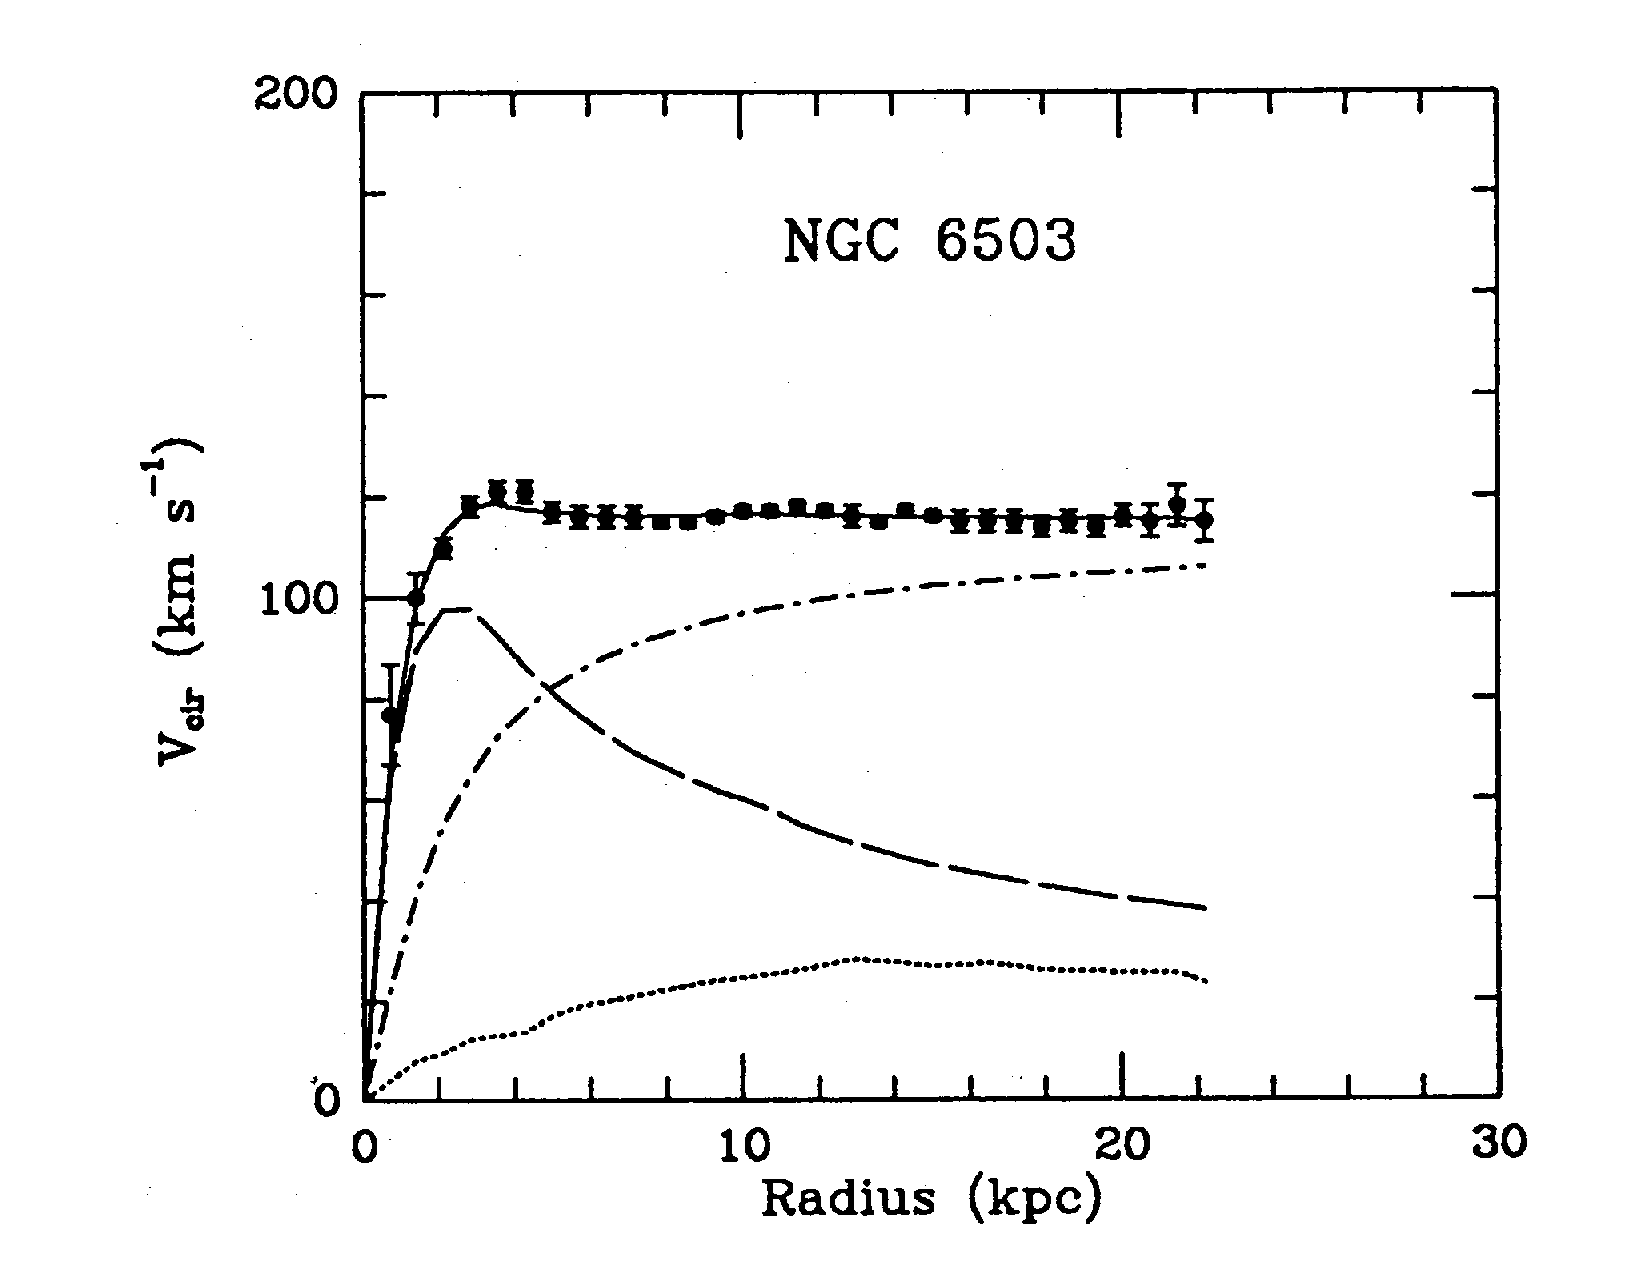
\includegraphics[height=0.45\textheight]{DMRotationalCurves}
			\caption[Galactic rotational velocity curve of NGC 6503.]{Galactic rotational velocity curve of NGC 6503
			from~\cite{Begeman:1991iy}.  The solid line is a three-component fit to the data with components from:
			visible mass (dashed), gas (dotted) and the dark halo (dash-dot).  }
			\label{fig:DMRotCurve}
		\end{figure}
	% WMAP results (large-scale structure)
	Other evidence of dark matter comes from measurements of large-scale structure through the analysis of the anisotropy of the cosmic microwave background (CMB) (see e.g.~\cite{Amsler20081}).  The extraction of cosmological parameters (e.g.~total matter density, baryon density, Hubble parameter, etc.) occurs by fitting the CMB data using model-based assumptions.  In particular, the parameters-of-interest are the total matter density, $\Omega_{m}$, and the baryon density, $\Omega_{b}$, which have been measured to be (in units of critical density):
		\begin{eqnarray*}
			\Omega_{m} & = & 0.256 \pm 0.02 \\
			\Omega_{b} & = & 0.044 \pm 0.003~\cite{Amsler20081}
		\end{eqnarray*}
If baryonic matter composed the majority of the mass in the universe, one would expect these two quantities to be equivalent.  Instead, the significant discrepancy between the two indicates the presence of unaccounted material.  Therefore, the dark matter component is the difference between these two components: $\Omega_{dm} = \Omega_{m} - \Omega_{b} = 0.21 \pm 0.02$, indicating a large proportion of dark matter in the universe on the order of 20\%.

	% Bullet cluster
	
	Perhaps the most visually stunning evidence for dark matter comes from the `bullet cluster' (galactic cluster 1E 0657-56)~\cite{Clowe06}.  In this particular example two subclusters have collided with one another $\sim$100~Myr ago, subjecting the contents of each to frictional forces.  The stars and galactic components of the subclusters were scarcely affected, passing through one another and interacting largely only gravitationally, but the trajectories of the hot gas making up the majority of the subclusters' baryonic mass density were significantly altered.  The matter density of the gas component was measured using images from the Chandra x-ray observatory and the total mass density of the cluster was measured using gravitational lensing.  When plots of these measurements are superimposed (see Figure~\ref{fig:DMBulletCluster} from~\cite{Clowe06}), it is clear that the two centers (of each subcluster) of the total mass density are offset from the centers of the gas-plasma mass density.  This indicates the presence of non-luminous (dark) matter weakly interacting with both the normal baryonic matter and with itself.  
	
			\begin{figure}
				\centering
				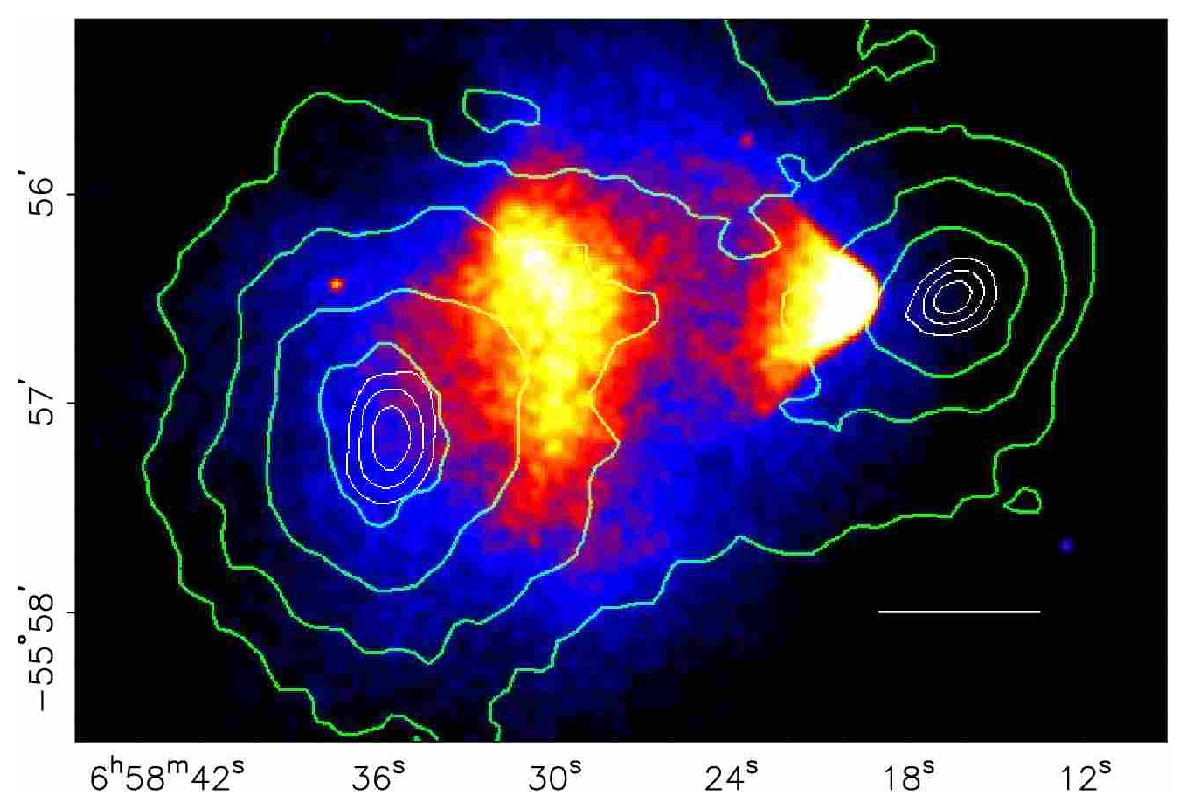
\includegraphics[height=0.45\textheight]{BulletCluster}
				\caption[Mass and x-ray image of the `bullet cluster', galactic cluster 1E 0657-56.]{Mass and x-ray image of 
				galactic cluster 1E 0657-56, 
				the `bullet cluster'.   The total mass, denoted by contour lines, has been measured using gravitational lensing; 
				the density of the gas, which composes the majority of the baryonic matter density in the cluster, has been 
				imaged using the Chandra x-ray observatory.  %The displacement of the centers of the total mass 
				Figure taken from reference~\cite{Clowe06}.}
				\label{fig:DMBulletCluster}
			\end{figure}	
	
	% Dark matter candidates	
		\subsection{Dark matter candidates}
	
	Whereas there are many particle candidates for dark matter, they share several general qualities:

	
	% Properties of Dark Matter particles
	% Stable
	% Interact poorly (or not at all) with electromagnetism
	% Should be non-relativistic (cold)
	
			\begin{enumerate}	
				\item Stable, having lifetimes at least on the order of the age of the universe.  Otherwise, dark matter would have
				decayed away.  
				\item Poor or no interaction with electromagnetism, making them non-luminous or `dark'.
				\item Non-relativistic at the time of galaxy formation: `hot' dark matter would move too quickly to clump, 
				not allowing it to affect large-scale structure formation as required by cosmological observation.  
			\end{enumerate}		

	% Looking at two species in particular:
	% WIMPs
	% Argument for WIMP dark matter: abundance considerations, freeze-out condition
Additionally, dark matter will compose a halo in our galaxy which the earth passes through as it transits around the sun.  Therefore, depending on the velocity dependence of the dark matter interaction, it is possible that the earth's orbit can generate an annual modulation in the dark matter signal, providing an additional distinguishing characteristic.  In the following, we will consider two potential species of dark matter in particular: WIMPs and axions. 
			\subsubsection{WIMPs}
 WIMPs, or Weakly-Interacting Massive Particles, (denoted from here on by $\chi$) are more of a class of candidate particles than one in particular, defined by the fact that these types of particles predominantly (or exclusively) interact via the weak force.  An argument for the existence of WIMPs relates to how they can `naturally' explain the dark matter relic abundance.
 % while making a few assumptions.  
  For example, during the period right after the big bang as the temperature of the universe was still quite hot, WIMPs would have been in equilibrium with other fermions, undergoing annihilation and generation according to the two-way reaction: $\chi\bar{\chi} \leftrightarrow f\bar{f} $ (see e.g.~Figure~\ref{fig:WIMPExampleProduction}).  As the temperature of the universe cooled below the mass of $\chi$, eventually this two-way process would shut off in one direction allowing only the interaction $\chi\bar{\chi} \rightarrow f\bar{f} $ to remain.  At this point in time, the rate of decay of $\chi$ has been calculated to be $\Gamma_{\chi} = \WIMPAnn n_{\chi}$~\cite{Jun96}, where $\sigma_{A}$ is the average cross-section for $\chi$ to annihilate into lighter fermions, $v$ is the average particle velocity, and $n_{\chi}$ is the density of WIMP particles.  The expansion of the universe would then reduce the density of $\chi$s, effectively shutting off this annihilation process and `freezing out' a so-called relic abundance of the particles.  

An estimate of the density of this abundance remaining today times the Hubble constant squared, $h^{2}\sim0.5$, can be calculated (see, e.g.~\cite{Jun96}):
			\begin{eqnarray}
				\Omega_{\chi} h^{2} & = & (2.6 \times 10^{-10}~\text{GeV}^{-2})~\WIMPAnn \\
				%\WIMPAnn & \sim & \frac{\alpha^{2}}{M_{\text{weak}}^{2}} \sim 10^{-9}~\text{GeV}^{-2}\\			
			\end{eqnarray}
and if we assume that this interaction follows the weak force, we can estimate the average cross section times the velocity as:
			\begin{eqnarray}
				%\Omega_{\chi} h^{2} & = & (2.6 \times 10^{-10}~\text{GeV}^{-2})~\WIMPAnn \\
				\WIMPAnn & \sim & \frac{\alpha^{2}}{M_{\text{weak}}^{2}} \sim 10^{-9}~\text{GeV}^{-2}\\			
			\end{eqnarray}
which leaves us with an estimate of 	$\Omega_{\chi} h^{2} \sim 0.2$, close to the observed cold-dark-matter density.  This realization has not been interpreted as a `coincidence' and instead is suggested as compelling support for the possibility of WIMP existence.  
		
			\begin{figure}
				\centering
				\def\figheight{0.4\textwidth}
				 \subfigure[WIMP annihilation and production] {
				 	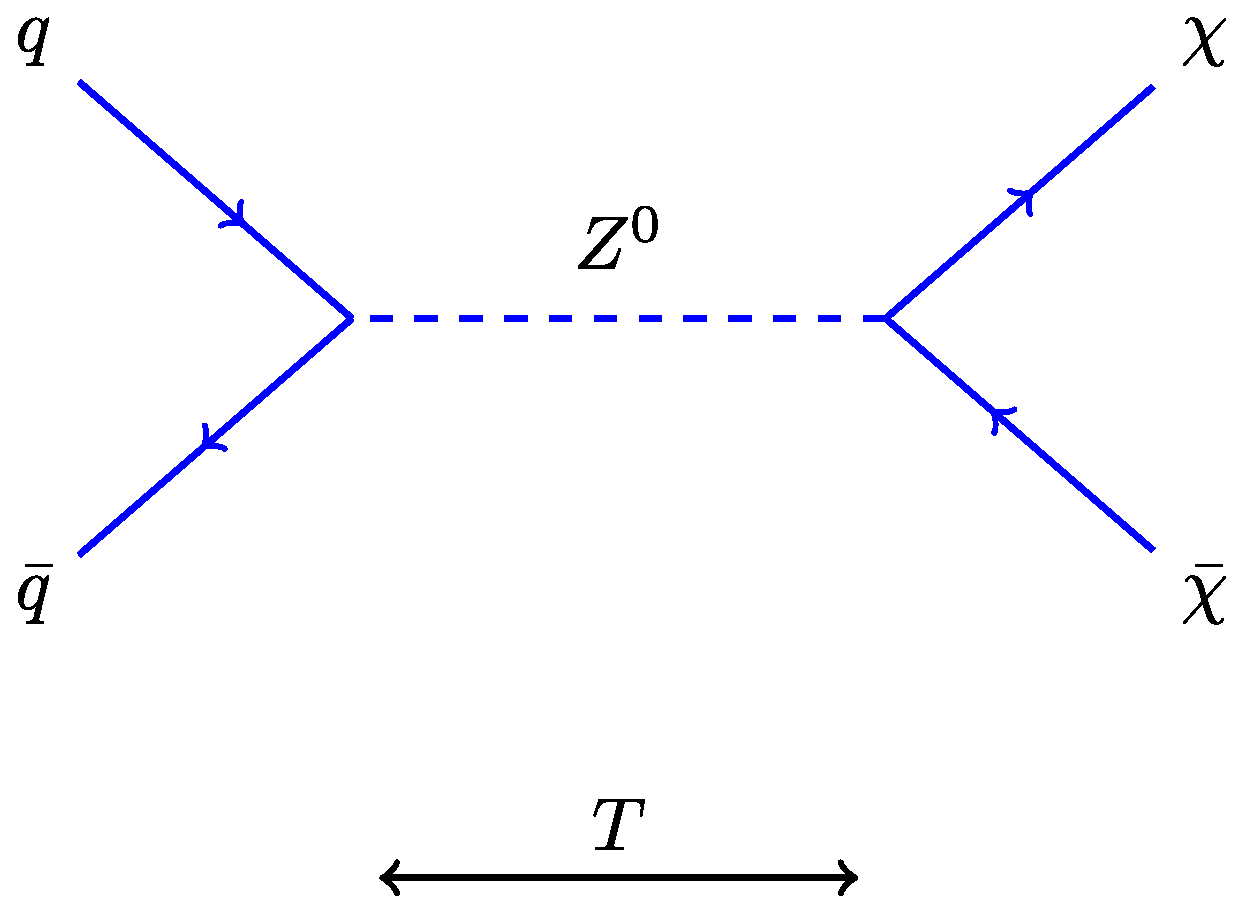
\includegraphics[width=0.6\textwidth]{WIMPProduction}
					\label{fig:WIMPExampleProduction}
				}
				\subfigure[WIMP elastic scattering]{
					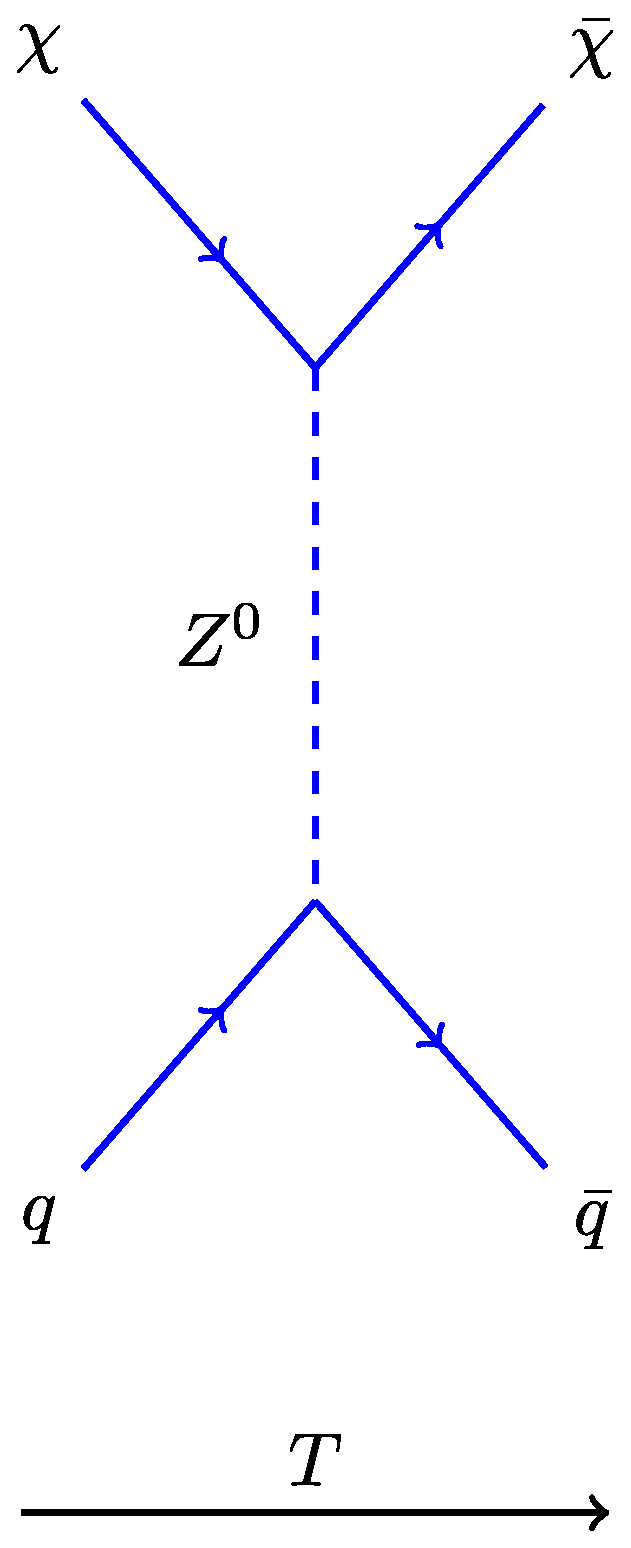
\includegraphics[width=0.25\textwidth]{WIMPScattering}
					\label{fig:WIMPExampleScattering}					
				}
				\caption[Relevant WIMP-quark interactions during hot and cold universe epochs.]{Example WIMP-quark 
				interactions mediated by the exchange of a $Z^{0}$ boson with the direction
				of time, $t$, indicated for each at bottom.  The left figure is applicable for WIMPs undergoing annihilation and 
				generation during the equilibrium phase at
				the beginning of the universe, when the temperature of the universe was much greater than the mass of $\chi$.
				The right figure denotes a mathematically equivalent interaction, an elastic-scattering process
				of $\chi$s off of quarks becoming relevant as the temperature of the universe reduced below the mass of $\chi$.}
				\label{fig:WIMPExample}
			\end{figure}	
			
	The direct detection of WIMPs is possible via their elastic scattering off of fermions, see e.g.~Figure~\ref{fig:WIMPExampleScattering}.  In creating a detector, we are of course generally limited to composing it out of electrons, neutrons, and protons.  In principle, WIMPs could scatter off of any fermion sharing a coupling to a mediating boson, but the kinematics of such a non-relativistic recoil maximize the energy transfer when the target particle has mass comparable to that of the incident particle.  In the case of WIMPs with hypothesized masses $\sim1\to1000$~GeV, an energy transfer is maximized during coherent recoil off of a nucleus having similar or equal mass.  Additionally, WIMP scattering off of bound electrons is suppressed due the mass ratio $m_{e}/m_{\chi}$, as well as the small size of the electronic wave function (see e.g.~\cite{Kopp09}) making the nuclear recoil the expected primary method of detection.  The standard form of the energy spectrum for a WIMP-induced nuclear recoil is outlined later in Section~\ref{sec:CalcLimitsOnWIMPSignal}.
	
			\subsubsection{Axions}
			\label{sec:AxionsAsDM}
	% Axions
	% Arguments for axions:
	% pseudoscalar bosons
	% Peccei-Quinn model - preserve CP in QCD 
	
	Axions are light, pseudoscalar bosons that were originally suggested as a mechanism to solve the CP problem of QCD~\cite{Pec77}.  In particular, the QCD Lagrangian includes a CP-violating term:
			\[
			\mathcal{L}_{\Theta} = \bar{\Theta} \frac{\alpha_s}{8 \pi} G^{\mu \nu a} \tilde{G}_{\mu \nu}^{a}
			\]
where $\Theta$ is an angle with possible value between $-\pi$ and $\pi$.  The lack of experimental evidence for CP violation in QCD suggests that this value is very small or 0, an `unnatural' solution given its range of possible values.  The Peccei-Quinn mechanism was proposed~\cite{Pec77} to explain this issue by adding an additional $U(1)_{PQ}$ symmetry to the Lagrangian.  The breaking of this symmetry results in a Nambu-Goldstone boson -- the axion -- updating the CP-violating portion of the QCD Lagrangian to be:
			\[
			\mathcal{L}_{\Theta} = \left( \bar{\Theta} - \frac{\phi_{A}}{f_{A}}\right) \frac{\alpha_s}{8 \pi} G^{\mu \nu a} \tilde{G}_{\mu \nu}^{a}
			\]	
with $\phi_{A}$ the axion field and $f_{A}$ the axion decay constant~\cite{Amsler20081}.  The expectation value of the axion is found to be $\phi_{A} = f_{A} \bar{\Theta}$ thereby directly canceling the CP violating term.  
	
	Bounds on axion properties can derive from cosmological observations as well as direct experimental searches.  For example, cosmological data can constrain axion models by looking for the evidence of additional unexplained energy loss in stars (see, e.g.~\cite{Gondolo09,Raf96}).  Direct detection measurements may take advantage of axions coupling with 2~photons, looking for their interaction in high-intensity magnetic fields, as is the case with the CAST experiment~\cite{Arik09} searching for axions produced in the sun, or searching for an axion interaction in a resonant microwave cavity within a magnetic field, as does the ADMX experiment~\cite{Asz10}.  Germanium detectors are not ideal for searching for such a signal, but can put bounds on the strength of the axion's coupling with electrons by searching for the inelastic scattering of an axion off of an electron.  This interaction and the observed signal is discussed in more detail in Section~\ref{sec:CalcLimitsOnHeavyAxionSignal}.
		
		\subsection{\ppc~detectors and dark matter}

	
	% WIMPs, truncated exponential
	
	\ppc~detectors can provide excellent dark matter detectors due to their low-energy threshold ($O(100~\text{eV})$) and excellent resolution down to threshold.  This can be made more clear if we consider the signal that WIMPs and axions can leave in a germanium detector.  These signals and their exact spectral form are discussed in more detail later for WIMPs (see Section~\ref{sec:CalcLimitsOnWIMPSignal}) and axions (see Section~\ref{sec:CalcLimitsOnHeavyAxionSignal}), but we consider their general properties here.  
	
	The nuclear recoil signal from a WIMP is essentially described as an exponential in energy space truncated by the finite escape velocity of the WIMP from the halo (see, e.g.~\cite{Jun96, Lew96}).  The exponential constant is determined by the mass of the WIMP and the spectrum becomes steeper as the mass gets smaller.  This can be visualized in Figure~\ref{fig:WIMPDiffMasses}.  It is clear that lowering the threshold of the germanium detector is critical to detecting low-mass WIMPs, due to the steepening of the curves and the truncation of the signal.  The sub-keV thresholds of \ppc~detectors therefore enables sensitivity to these low masses.  Most WIMP experiments rely on the ability to distinguish between electron and nuclear recoils for background reduction since the vast majority of backgrounds (e.g.~gammas, alphas, and betas) interact solely with electrons.  \ppc~detectors will be unable to distinguish between these two types of events, instead relying on the passive reduction of radioactivity through the choice of radiopure materials and appropriate shielding.
	
			\begin{figure}
				\centering
				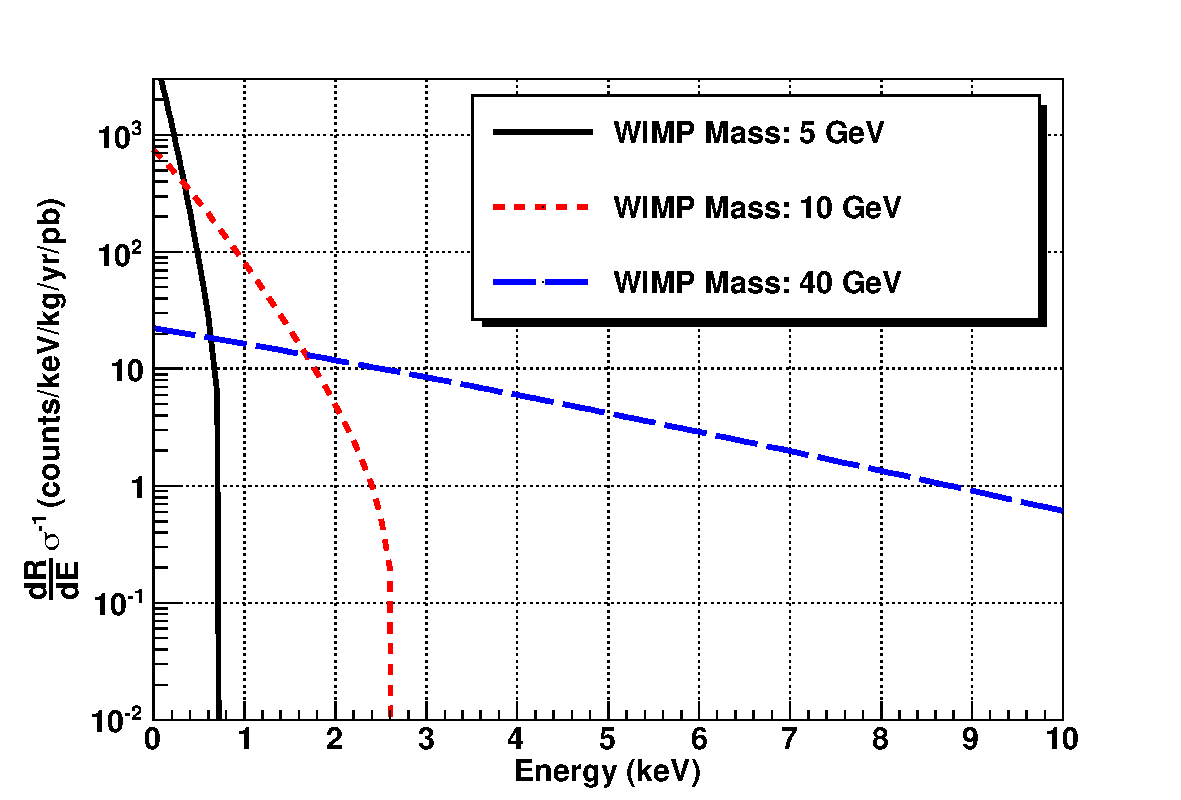
\includegraphics[width=0.9\textwidth]{WIMPModelCompareDiffMasses}
				\caption[Ionization spectrum of a WIMP nuclear-recoil in a Ge detector.]
				{Ionization spectrum (differential rate vs.~energy) of a WIMP nuclear-recoil in a Ge detector normalized by the
				 interaction cross section.  The signal becomes steeper with lower WIMP mass and the truncation due to the
				 escape velocity is more apparent at low mass.  Because of the characteristics of the signal, a germanium
				  detector with threshold greater than 1~keV could not detect a recoiling WIMP of mass 5~GeV, underscoring
				  the need for low thresholds to detect low-mass WIMPs.}
				\label{fig:WIMPDiffMasses}
			\end{figure}

	% Axioelectric effect - gaussian signal

	The signal for a non-relativistic axion interacting via the axioelectric effect has been derived in~\cite{Pospelov:2008jk}.  This particular inelastic interaction involves the deposition of the \emph{complete} energy of the axion, yielding an electron-recoil signal centered at the mass of the axion.  The low noise of \ppc~detectors yields excellent sensitivity to non-relativistic axions with masses $\leq10$~keV due their sharp resolution at low energies.  This enhanced performance is especially clear when compared to the capabilities of NaI scintillation detectors.  A comparison of an axioelectric signal at a defined axion-electron coupling ($\gaa$) is provided in Figure~\ref{fig:ResCompare} for characteristic resolutions of NaI and germanium detectors.  In this plot, it is clear that the improved resolution of the germanium detector allows less smearing of the signal, yielding more counts in a narrower peak.  This enhanced resolution enables superior distinction of the signal in the presence of background.
	
		\begin{figure}
			\centering
			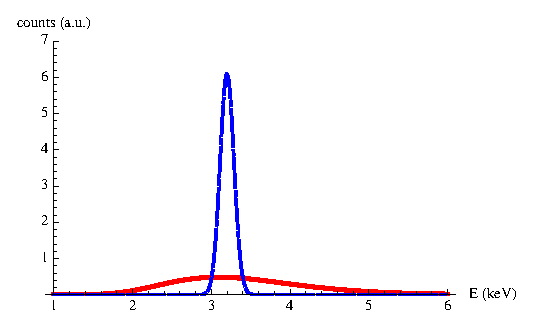
\includegraphics[width=0.9\textwidth]{DAMARes}
			\caption[Axion signal at $m_{a}$ = 3.2~keV]{Axion signal at $m_{a}$ = 3.2~keV comparing 
			the an estimate of detector responses of germanium (blue, dashed) and NaI (red, solid) to an equivalent
			axion-electron coupling ($\gaa$).}
			\label{fig:ResCompare}
		\end{figure}
	
	\section{Outline of this dissertation}

		% Development of a digital DAQ, understanding the needs to get a fully-functional DAQ able to satisfy both the requirements of nonubb and low-energy physics
		% Deployment of an initial detector and system underground, what we learned
		% A final system (with updated DAQ, etc.) underground
		% Limits on WIMPs and the axioelectric effect as well as considerations for Majorana

	This dissertation will focus on understanding and exploiting the low-energy capabilities of \ppc~detectors.  It will begin by considering the data acquisition (DAQ) needs to read out these detectors to enable full access to physics at $\qval$ and at low energies.  Following this will be the description of the application of this DAQ system to a \ppc~detector deployed underground at Soudan Underground Laboratory in Soudan, Minnesota, including conclusions from this initial study.  Results and knowledge gained from this initial detector were then applied to the deployment of another, lower-background \ppc~at Soudan.  The analysis of this detector, including the generation of limits for WIMP and axion dark matter, comprises the bulk of the thesis.  Finally, the work ends with some contextual discussion of these results, focusing on estimating the sensitivity of the \MJ~\minmod~to detect dark matter.  Appendices detailing the development and use of software for the results of this dissertation are included for reference.
